\documentclass[journal]{IEEEtran}
\usepackage[a5paper, margin=10mm, onecolumn]{geometry}
%\usepackage{lmodern} % Ensure lmodern is loaded for pdflatex
\usepackage{tfrupee} % Include tfrupee package

\setlength{\headheight}{1cm} % Set the height of the header box
\setlength{\headsep}{0mm}     % Set the distance between the header box and the top of the text

\usepackage{gvv-book}
\usepackage{gvv}
\usepackage{cite}
\usepackage{amsmath,amssymb,amsfonts,amsthm}
\usepackage{algorithmic}
\usepackage{graphicx}
\usepackage{textcomp}
\usepackage{xcolor}
\usepackage{txfonts}
\usepackage{listings}
\usepackage{enumitem}
\usepackage{mathtools}
\usepackage{gensymb}
\usepackage{comment}
\usepackage[breaklinks=true]{hyperref}
\usepackage{tkz-euclide} 
\usepackage{listings}
% \usepackage{gvv}                                        
\def\inputGnumericTable{}                                 
\usepackage[latin1]{inputenc}                                
\usepackage{color}                                            
\usepackage{array}                                            
\usepackage{longtable}                                       
\usepackage{calc}                                             
\usepackage{multirow}                                         
\usepackage{hhline}                                           
\usepackage{ifthen}                                           
\usepackage{lscape}
\begin{document}

\bibliographystyle{IEEEtran}
\vspace{3cm}

\title{11.16.3.3.1}
\author{EE24BTECH11064 - Harshil Rathan}
 \maketitle
% \newpage
% \bigskip
{\let\newpage\relax\maketitle}

\renewcommand{\thefigure}{\theenumi}
\renewcommand{\thetable}{\theenumi}
\setlength{\intextsep}{10pt} % Space between text and floats


\numberwithin{equation}{enumi}
\numberwithin{figure}{enumi}
\renewcommand{\thetable}{\theenumi}
\textbf{Question}:\\
A die is thrown, find the probability of following events : 
\begin{itemize}
    \item[i)] A prime number will appear 
\end{itemize}
\textbf{Theoretical Solution: }\\
The sample space $S$ of a fair six-sided die is
\begin{align}
    S = {1,2,3,4,5,6}
\end{align}
The prime numbers in the Sample space are 
\begin{align}
    A = {2,3,5}
\end{align}
Thus, the number of favorable outcomes = 3 
\begin{align}
    |S| = 6 
    \label{0.3}
\end{align}
\begin{align}
    |A| = 3 
    \label{0.4}
\end{align}
The probability of getting a prime number when a fair die is rolled
\begin{align}
    P(A) = \frac{|A|}{|S|}   
\end{align}
on substituing \ref{0.3}, \ref{0.4}
\begin{align}
    P(A) = \frac{1}{2}
\end{align}
\textbf{Computational solution: }\\

\section*{Computation of Probabilities for Rolling a Die}

To compute the probability of obtaining specific outcomes when rolling a six-sided die, we rely on two key concepts: the Probability Mass Function (PMF) and the Cumulative Distribution Function (CDF).

\subsection*{Definitions}
\subsubsection*{Probability Mass Function (PMF)}
The PMF represents the probability of each individual outcome in the sample space \( S \). For a six-sided die:
\[
S = \{1, 2, 3, 4, 5, 6\},
\]
the PMF is given as:
\[
P(X = x) = 
\begin{cases} 
\frac{1}{3}, & x \in \{2, 3, 5\}, \\ 
0, & x \notin \{2, 3, 5\}.
\end{cases}
\]

\subsubsection*{Cumulative Distribution Function (CDF)}
The CDF represents the cumulative probability of outcomes up to a given value \( x \), defined as:
\[
F(x) = P(X \leq x) = \sum_{k=1}^{x} P(X = k).
\]
For the event "A prime number will appear" on a six-sided die:
\[
F(x) = 
\begin{cases} 
0, & x < 2, \\
\frac{1}{3}, & 2 \leq x < 3, \\
\frac{2}{3}, & 3 \leq x < 5, \\
1, & x \geq 5.
\end{cases}
\]

\subsection*{Simulation Process}
We simulate the rolling of a die to compute the probability of a prime number appearing using the following steps:
\begin{enumerate}
    \item A six-sided die produces outcomes in the set:
    \[
    S = \{1, 2, 3, 4, 5, 6\}.
    \]
    \item Identify the subset of outcomes corresponding to prime numbers:
    \[
    S_{\text{prime}} = \{2, 3, 5\}.
    \]
    \item For each simulated roll, a random integer \( X \) is generated such that \( X \in S \), using a random number generator function:
    \[
    X = (\text{rand()} \mod 6) + 1.
    \]
    \item Check if the outcome \( X \in S_{\text{prime}} \). Track the number of occurrences of prime outcomes over \( N \) trials, where \( N \) is the total number of simulations.
    \item Compute both the PMF and CDF for the event "A prime number appears":
    \begin{itemize}
        \item PMF: The frequency of each prime outcome (\( \{2, 3, 5\} \)) is divided by the total trials to compute the probability of each prime face. Non-prime outcomes (\( \{1, 4, 6\} \)) have probabilities of zero.
        \item CDF: The cumulative probabilities are calculated by summing the PMF values of the prime outcomes up to a given \( x \). For \( x \notin S_{\text{prime}} \), the CDF remains constant.
    \end{itemize}
\end{enumerate}

\subsection*{Calculation of Probabilities}

\subsubsection*{Probability of Each Outcome (PMF)}
The probability of rolling each face \( i \) (\( i \in \{2, 3, 5\} \)) is computed as:
\[
P(i) = \frac{\text{Number of rolls resulting in } i}{N},
\]
where \( i \) is restricted to the set of prime numbers \( \{2, 3, 5\} \). For non-prime outcomes (\( i \in \{1, 4, 6\} \)), \( P(i) = 0 \).

\subsubsection*{Cumulative Probability (CDF)}
The cumulative probability up to face \( i \) is:
\[
F(i) = 
\begin{cases} 
0, & i < 2, \\
\frac{1}{3}, & 2 \leq i < 3, \\
\frac{2}{3}, & 3 \leq i < 5, \\
1, & i \geq 5.
\end{cases}
\]
Here, \( F(i) \) accumulates probabilities only for the prime outcomes. For non-prime values of \( i \), \( F(i) \) remains constant.

\subsection*{Output Representation}
The computed probabilities are represented in two forms:
\begin{itemize}
    \item \textbf{PMF}: The probabilities of rolling each face from the set of prime numbers \( \{2, 3, 5\} \). Non-prime outcomes \( \{1, 4, 6\} \) have probabilities of zero.
    \item \textbf{CDF}: The cumulative probabilities up to each face \( \{2, 3, 5\} \), showing the cumulative likelihood of rolling a prime number. For non-prime outcomes, the cumulative probability remains constant.
\end{itemize}

\section*{Stemplot Distribution}
When a die is rolled, the prime outcomes are ${2,3,5}$. Each face of a fair die has an equal probability of occurring, which is $\frac{1}{6}$. This means that each of the outcomes {2,3,5} have probability $\frac{1}{6}$
\begin{itemize}
    \item The stem plot shows vertical lines (stems) at the positions 2, 3, 5 on the x-axis 
    \item The height of each stem corresponds to the probability of that particular prime number outcome $\frac{1}{6}$
\end{itemize}
\begin{align}
    P(A) = P(2) + P(3) + P(5) = \frac{1}{6}+\frac{1}{6} +\frac{1}{6} = \frac{1}{2}
\end{align}
\section*{Conclusion}
This task demonstrates the integration of C and Python for simulating and visualizing a probabilistic experiment. By combining the computational efficiency of C with the graphical capabilities of Python, we achieve an effective solution for analyzing and representing data. The code clearly shows that the probability of the given event is equal to \textbf{half}
\begin{figure}[h!]
   \centering
   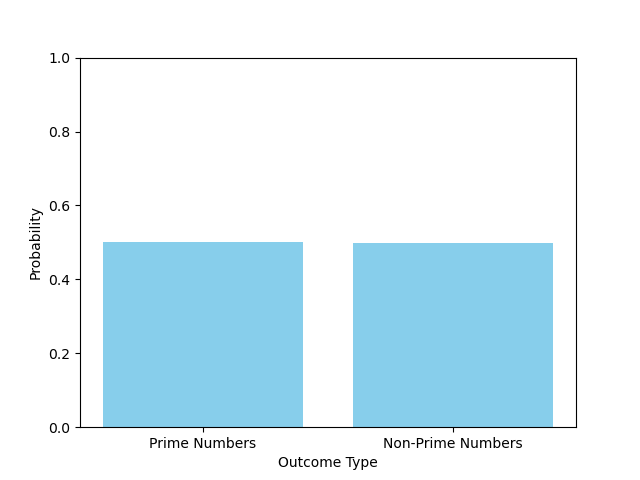
\includegraphics[width=\columnwidth]{figs/Figure_1.png}
\end{figure}
\begin{figure}[h!]
   \centering
   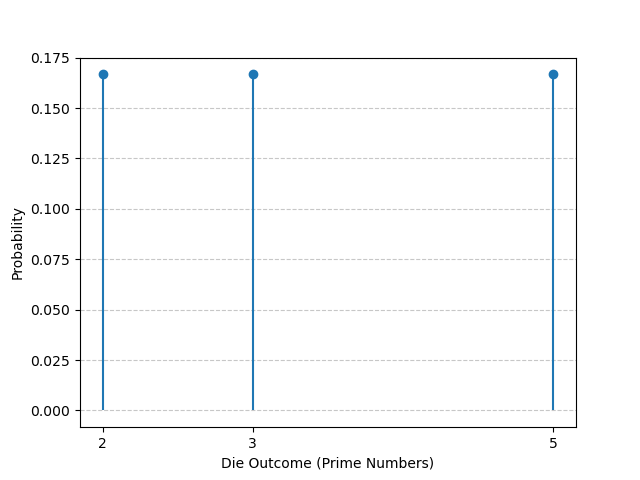
\includegraphics[width=\columnwidth]{figs/Figure_2.png}
\end{figure}
\end{document}
